\subsection{Practices and standards}

The \gls{G19} tries to uphold a set of practices and standards found in the process manual \cite{processManual}. This section describes the categories of the practices and standards, which are:

\begin{itemize}
    \item Coding standards
    \item Documentation standards
    \item Version control
    \item Code review
\end{itemize}

\subsubsection{Coding Standards}

The coding standards involve naming conventions, descriptions, and a few other aspects. The motivation behind coding standards is to make the code easier to read.

We found it especially hard to get to know the Weekplanner application when we were handed its source code because it seemed like they lacked a strict coding standard.

\subsubsection{Documentation}

The process manual also states that when a \gls{devTeam} implements a user story, they should document the workings of each component created to fulfill that user story, both in terms of responsibility and how it interacts with the rest of the system, which should lead to a comprehensive system description.

When a developer identifies a bug or other shortcomings of the system, they should file a report in the issue tracker which enables systematic documentation of errors. The \gls{POT} filters through these issues, and from them creates user stories.

\subsubsection{Version Control}

A strict strategy for version control, namely GitFlow \cite{GitFlow}, was enforced to ensure that all developers utilized the version control similarly. GitFlow is a Git Workflow framework originally published by Vincent Driessen, the aim of which is to manage large scale projects \cite{GitFlow}.

The way GitFlow manages large scale projects is with strict branching rules, dictating the allowed branch types for the projects \cite{GitFlow} as described below:

\begin{itemize}
    \item One master branch - this is the branch where the most recent release is, every commit to this branch is a new release.
    \item One develop branch - based on the master branch; this is the branch where active development merges. The develop branch is never merged into other branches.
    \item A set of feature branches - every feature should have a branch, which is based on the develop branch and should merge back into the develop branch when finished.
    \item A set of release branches - scheduling a release or when there are enough new features in the develop branch constitutes a need for a release branch. Release branches fork out of the develop branch. This branch is not allowed to have any feature-branches merged into it, only bug fixes. When the release branch is stable, it is merged into master and thereby becoming the newest release.
    \item A set of hotfix branches - Fixing a bug in the current master branch constitutes a need for a hotfix branch, which is forked out of the master branch and merges into both the master and develop branch.
\end{itemize}

\Gls{G19} adopted this framework into the \gls{giraf} project \cite{ProcessGitFlow} but with some deviations from the standard GitFlow framework. These deviations are:

\begin{itemize}
    \item A feature branch is to be squashed and merged with the develop branch, which ensures that every feature is only one commit in the develop branch.
    \item We fork release branches off the master branch and cherry-pick the relevant features for this release branch from the develop branch. Cherry-picking is when one merges a specific subset of commits from one branch to another.
    \item Hotfixes merge into the release branch.
    \item The release branch is merged into the master and develop branch.
\end{itemize}

\begin{figure}[H]
        \begin{center}
            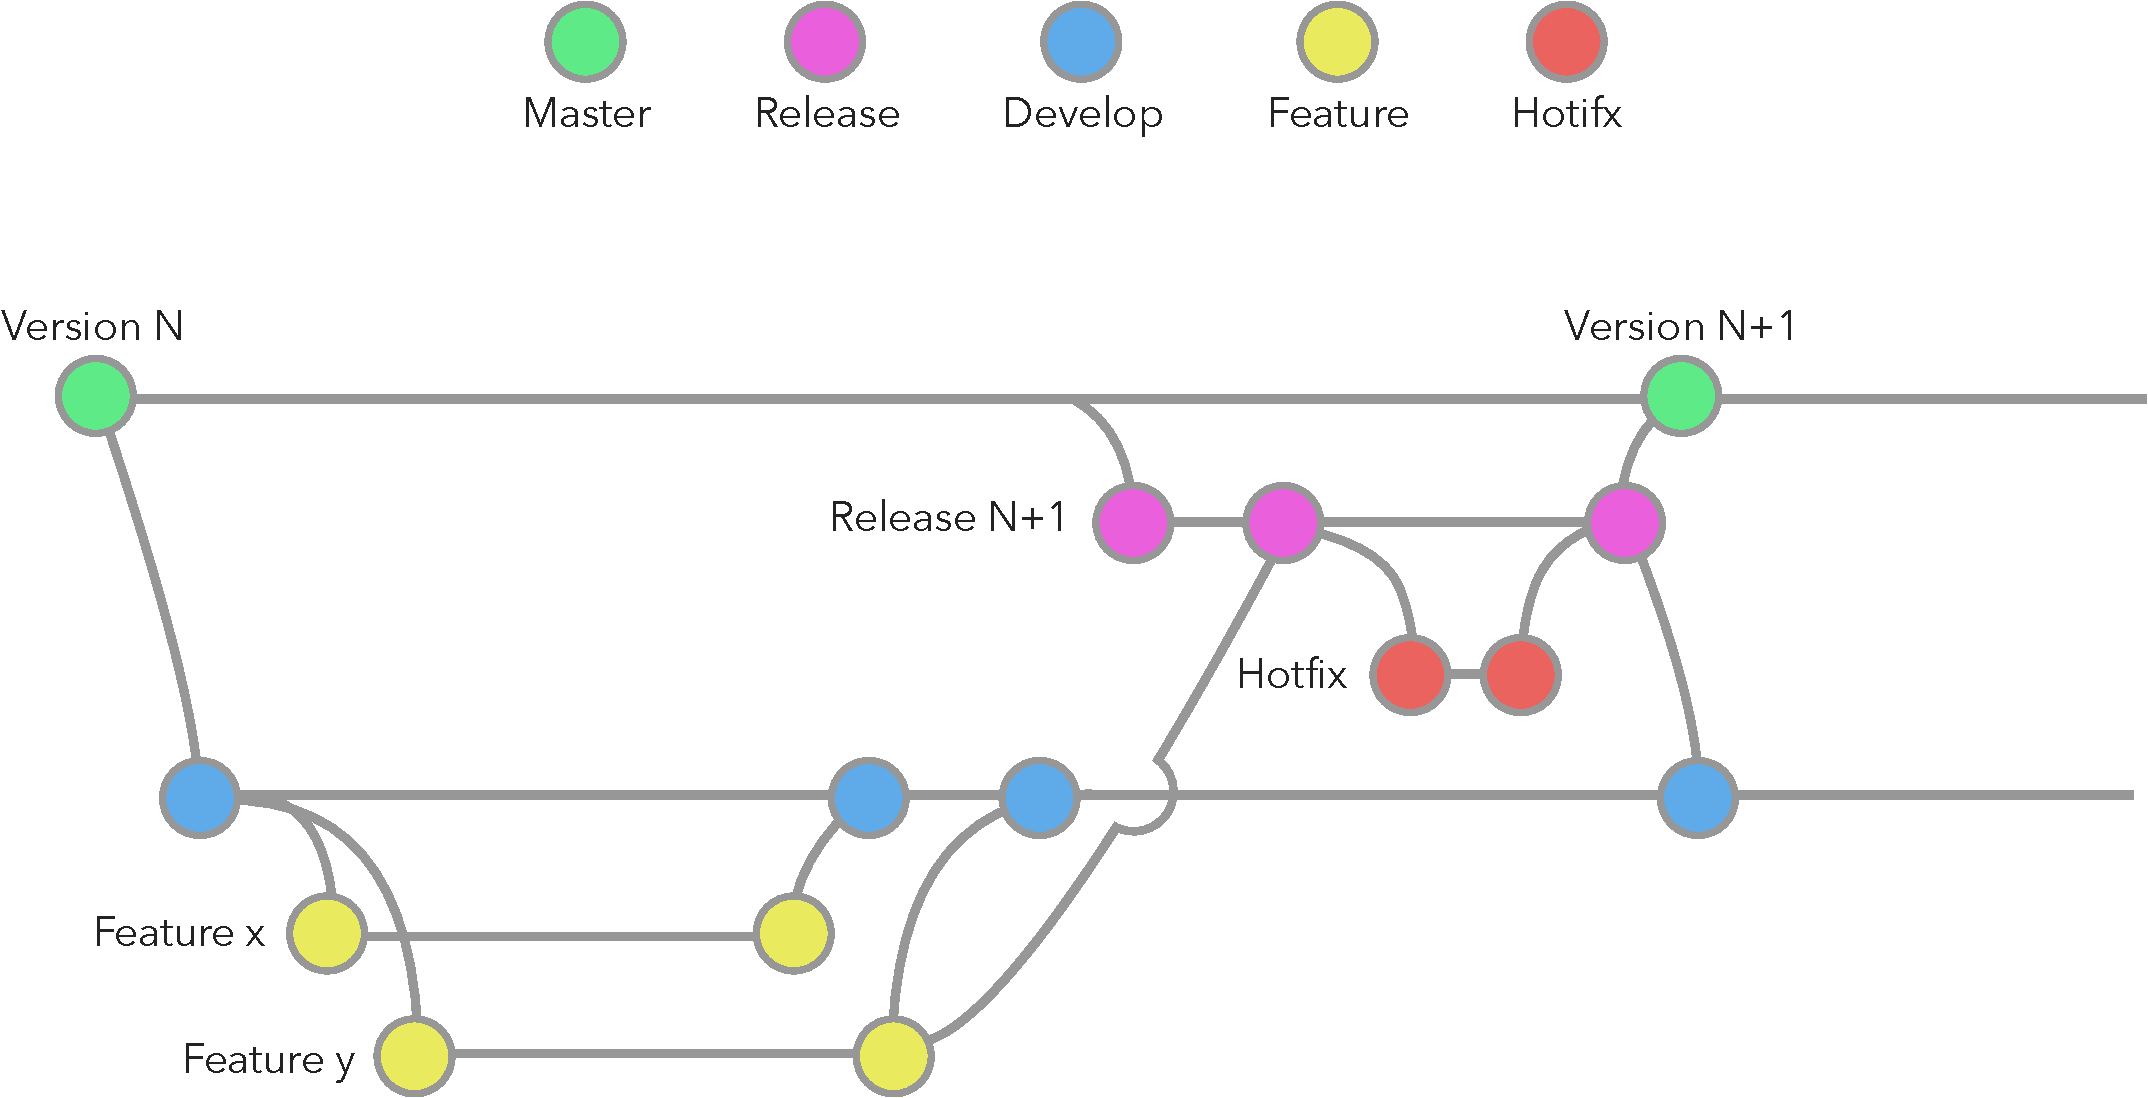
\includegraphics[width=0.95\textwidth]{figures/gitflow_overview.pdf}
        \end{center}
        \caption{An illustration of the \gls{giraf} adaptation of GitFlow}
        \label{fig:girafgitFlowfigure}
\end{figure}

\autoref{fig:girafgitFlowfigure} illustrates \gls{giraf}'s adaptation of the GitFlow. \autoref{fig:girafgitFlowfigure} shows how \textit{Feature y} is cherry-picked, and \textit{Feature x} is not.
